\section{Introduction}
\label{sec:intro}

Writing a Geant4\cite{geant4} simulation application with no hardcoded numbers is
as easy as replacing calls such as~\verb|G4Box(‘box’, 20, 30, 40)| with
code like~\verb|G4Box(name, a, b, c)|
where the parameters are read from a database, for example mysql.
This however is not particularly useful: users still need to write C++ and Geant4 code to setup
the volumes definitions organization, sensitivity, how to digitized the Geant4 steps
and collect them into hits, then save those hits in the output.

\begin{figure}[h]
    \centering
    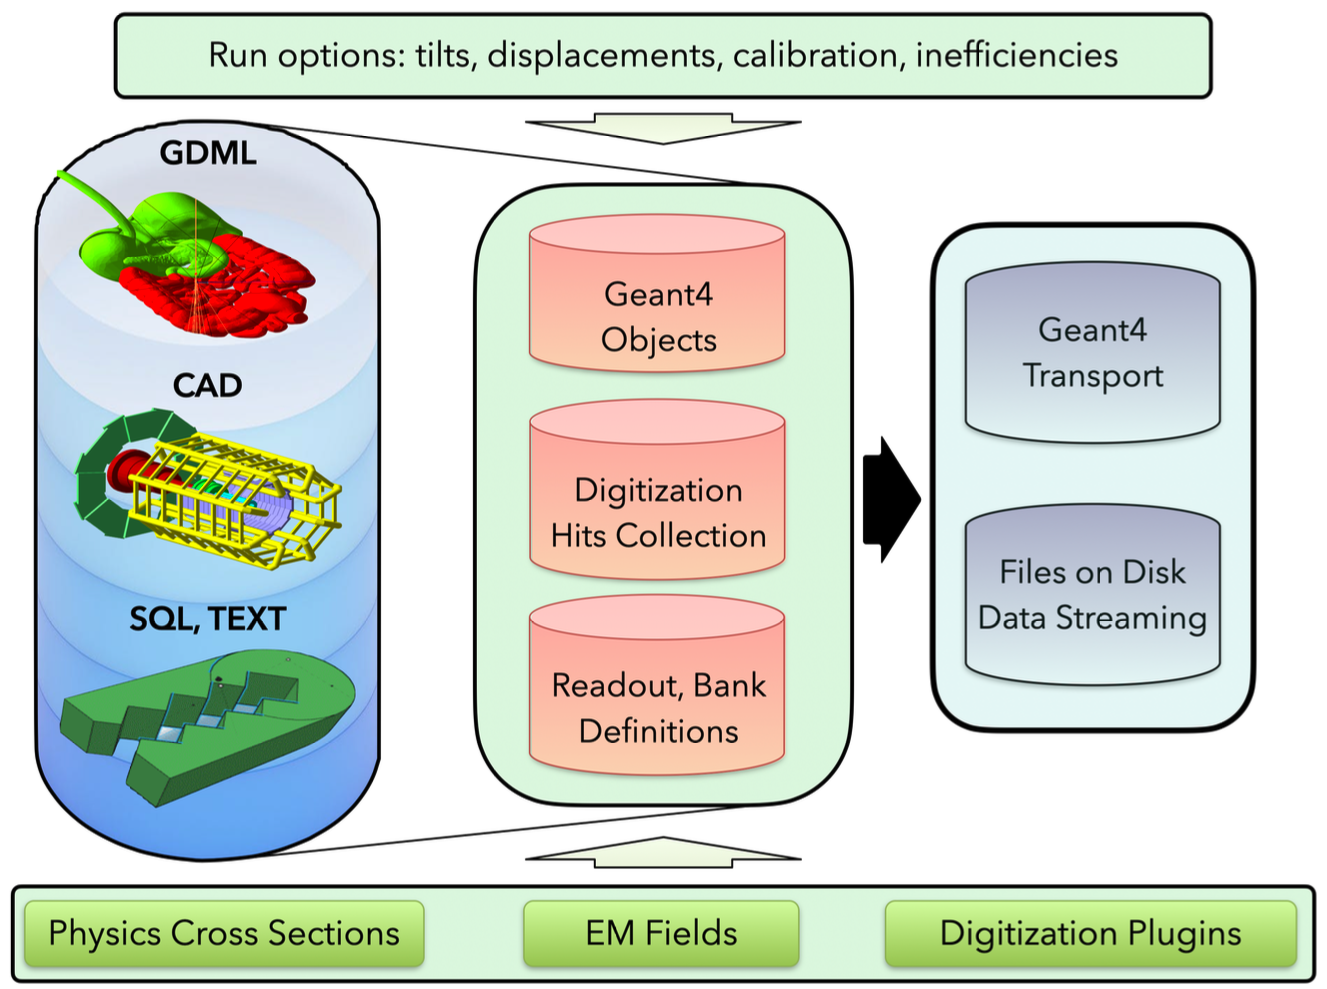
\includegraphics[width=.95\textwidth]{img/db}
    \caption{GEMC: a Geant4 application driven in its entirety by databases: geometry, materials,
        digitization, readout electronics, output format. Additional configurations such as which phusics
        list to use, magnetic field, which experment to run can be provided by steering cards (JSON).}
    \label{fig:db}
\end{figure}

A program such as the one sketched Fig.\ref{fig:db}, capable of driving in its entirety
a Geant4 simulation from databases and steering cards present several advantages:

\begin{itemize}
    \item no pre-requisite knowledge of C++ or Geant4 required to write the simulation:
    users can focus on geometry by interacting with the databases
    \item the experiment setup is naturally shared among different users,
    without the need to re-compile  the code
    \item the same application can be used to simulate different experiments,
    by simply selecting the desired setup from the database
\end{itemize}

We present the database driven GEMC\cite{clas12_gemc, gemc_homepage} application.
It provides:

\begin{itemize}
    \item an intuitive python API to build detectors and populate the databases
    \item CAD (STL) and GDML import
    \item hardware emulation of the readout electronics
    \item user defined digitization of the Geant4 steps
    \item data streaming to disk or network
\end{itemize}


\section{Features}
\label{sec:features}

\subsection{Geometry Sources}
\label{subsec:databases}
GEMC can read geometry and materials definitions from several sources:
\begin{itemize}
    \item CAD import: each object is defined by a STL file.
    The directory containing the files is loaded by the steering card.
    An optional JSON file can provide additional attributes to each volume,
    such as materials, hierarchy, position, rotation, etc.
    \item GDML files: same as CAD import, but the geometry is defined
    in a GDML file.
    \item MySQL, Sqlite databases, text files. Native geant4 geometry
    and materials are defined by the python API and saved in either
    a database or a text file. This includes copies and boolean operations
    between volumes defined by the other sources.
\end{itemize}
The hierarchy of the volumes is defined by the user and can be mixed between
the different sources. For example, a CAD file can be imported and then be the parent
of a volume defined in a database, or viceversa.

\subsection{Python API}
\label{subsec:api}
The python API is used to build the detectors and populate the databases.
The API is written with the goal of being intuitive and easy to use,
and it is the only code that needs to be written to  develop a simulation.
The code below defines a cylindrical target and a sensitive 'flux' detector.

% insert python code here
\begin{lstlisting}[language=Python]
gvolume = GVolume('target')
gvolume.description = 'Liquid Hydrogen Target'
gvolume.make_tube(0, 20, 40, 0, 360)
gvolume.material    = 'G4_lH2'
gvolume.color       = 'ff0000'
gvolume.publish(configuration)

gvolume = GVolume('paddle')
gvolume.description = 'Scintillator paddle'
gvolume.make_box(5, 0.5, 5, 'cm')
gvolume.material = 'G4_PLASTIC_SC_VINYLTOLUENE'
gvolume.set_rotation(90, 0, 0)
gvolume.set_position(0, 2, 10, 'cm')
gvolume.color        = 'f4f4ff'
gvolume.digitization = 'flux'
gvolume.set_identifier('paddleid', 5)
gvolume.publish(configuration)
\end{lstlisting}

This is the only code that needs to be written to define the geometry and materials.

The resulting setup example is shown in Fig.\ref{fig:api}.

\begin{figure}[h]
    \centering
    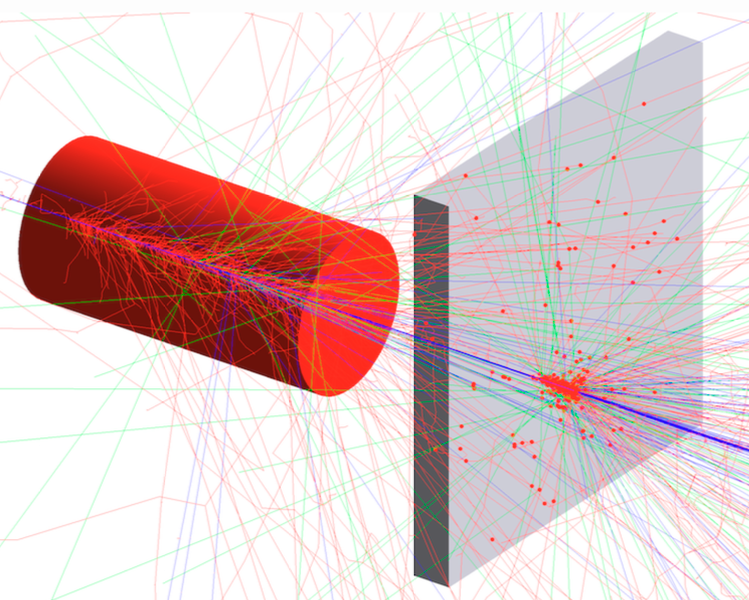
\includegraphics[width=.95\textwidth]{img/api}
    \caption{Example of the python API to build a detector and populate the databases.
        The API is written with the goal of being intuitive and easy to use,
        and it is the only code that needs to be written to  develop a simulation.}
    \label{fig:api}
\end{figure}


\subsection{Electronic Time Window}
\label{subsec:time_window}

\subsection{Energy Sharing}
\label{subsec:energy_sharing}

\subsection{Sensitivity and Digitization}
\label{subsec:digitization}



\subsection{Data Streamer}
\label{subsec:data_streamer}


\section{Examples}
\label{sec:examples}

\subsection{Cad Import}
\label{subsec:cad_import}

\subsection{Flux scintillator paddle}
\label{subsec:flux_scintillator_paddle}

\subsection{GEMC at Jefferson Lab}
\label{subsec:clas12}


\section{Summary}
\label{sec:summary}

